\begin{comment}
Background
 - Smallsats
 - Mission planning and execution
 - Current telemetry display solutions
   - Large custom-made software suites, single-purpose - large time requirements for implementation and change

Motivation
 - NTNU SmallSat/HYPSO
 - Spacecraft telemetry
 - How should one display and process telemetry?
 - Why Open MCT works for this
   - Open framework, used by NASA on multiple projects; one of the few frameworks of its type that’s available to the public
   -Wanted to implement a well-documented and expandable solution for this; Open MCT has few existing implementations, as it is a fairly new framework - largely minor modifications of the tutorial
\end{comment}

\section{Introduction}

The HYPSO project at NTNU SmallSats is in need of a system for displaying and working with telemetry data from the satellite.

Current space telemetry visualisation systems are often large monoliths of closed-source software written exclusively for one system with limited potential for modification or reuse without extensive rewrites. One major exception to this is the recently emerging Open Mission Control Technologies framework from NASA and JPL, which provides an interesting opportunity for trying out a new and more flexible approach to telemetry visualisation.

The goal of this project assignment is to use this new framework to build a telemetry data visualisation system for the HYPSO satellite, and investigate if it is a good fit for the HYPSO team as a telemetry visualisation system.

This report will start with quick introductions to what telemetry, Open MCT and HYPSO are, followed by an overview of the requirements and inputs plus outputs for the system we need to implement to get data from the HYPSO satellite into Open MCT. After this a design specification draft for a possible initial version of the system will be documented and discussed, before covering to the process, design changes and final results of implementing a functional version of the planned system.

\section{Background}

\subsection{Telemetry basics}
Satellites and other spacecraft produce a fairly significant amount of data that needs to be processed on a day-to-day basis. The part of this that is sent to a ground station via a wireless communication link is what's commonly referred to as \gls{telemetry} in the space industry. Some of this data may be unique to the mission of the spacecraft, such as image data from a camera or a measurement from a scientific instrument. However, in many cases the most important data for the ground-based operators is the telemetry data that lets them gauge the current status of the spacecraft and subsequently plan future missions and actions for it.

\begin{figure}[H]
    \centering
    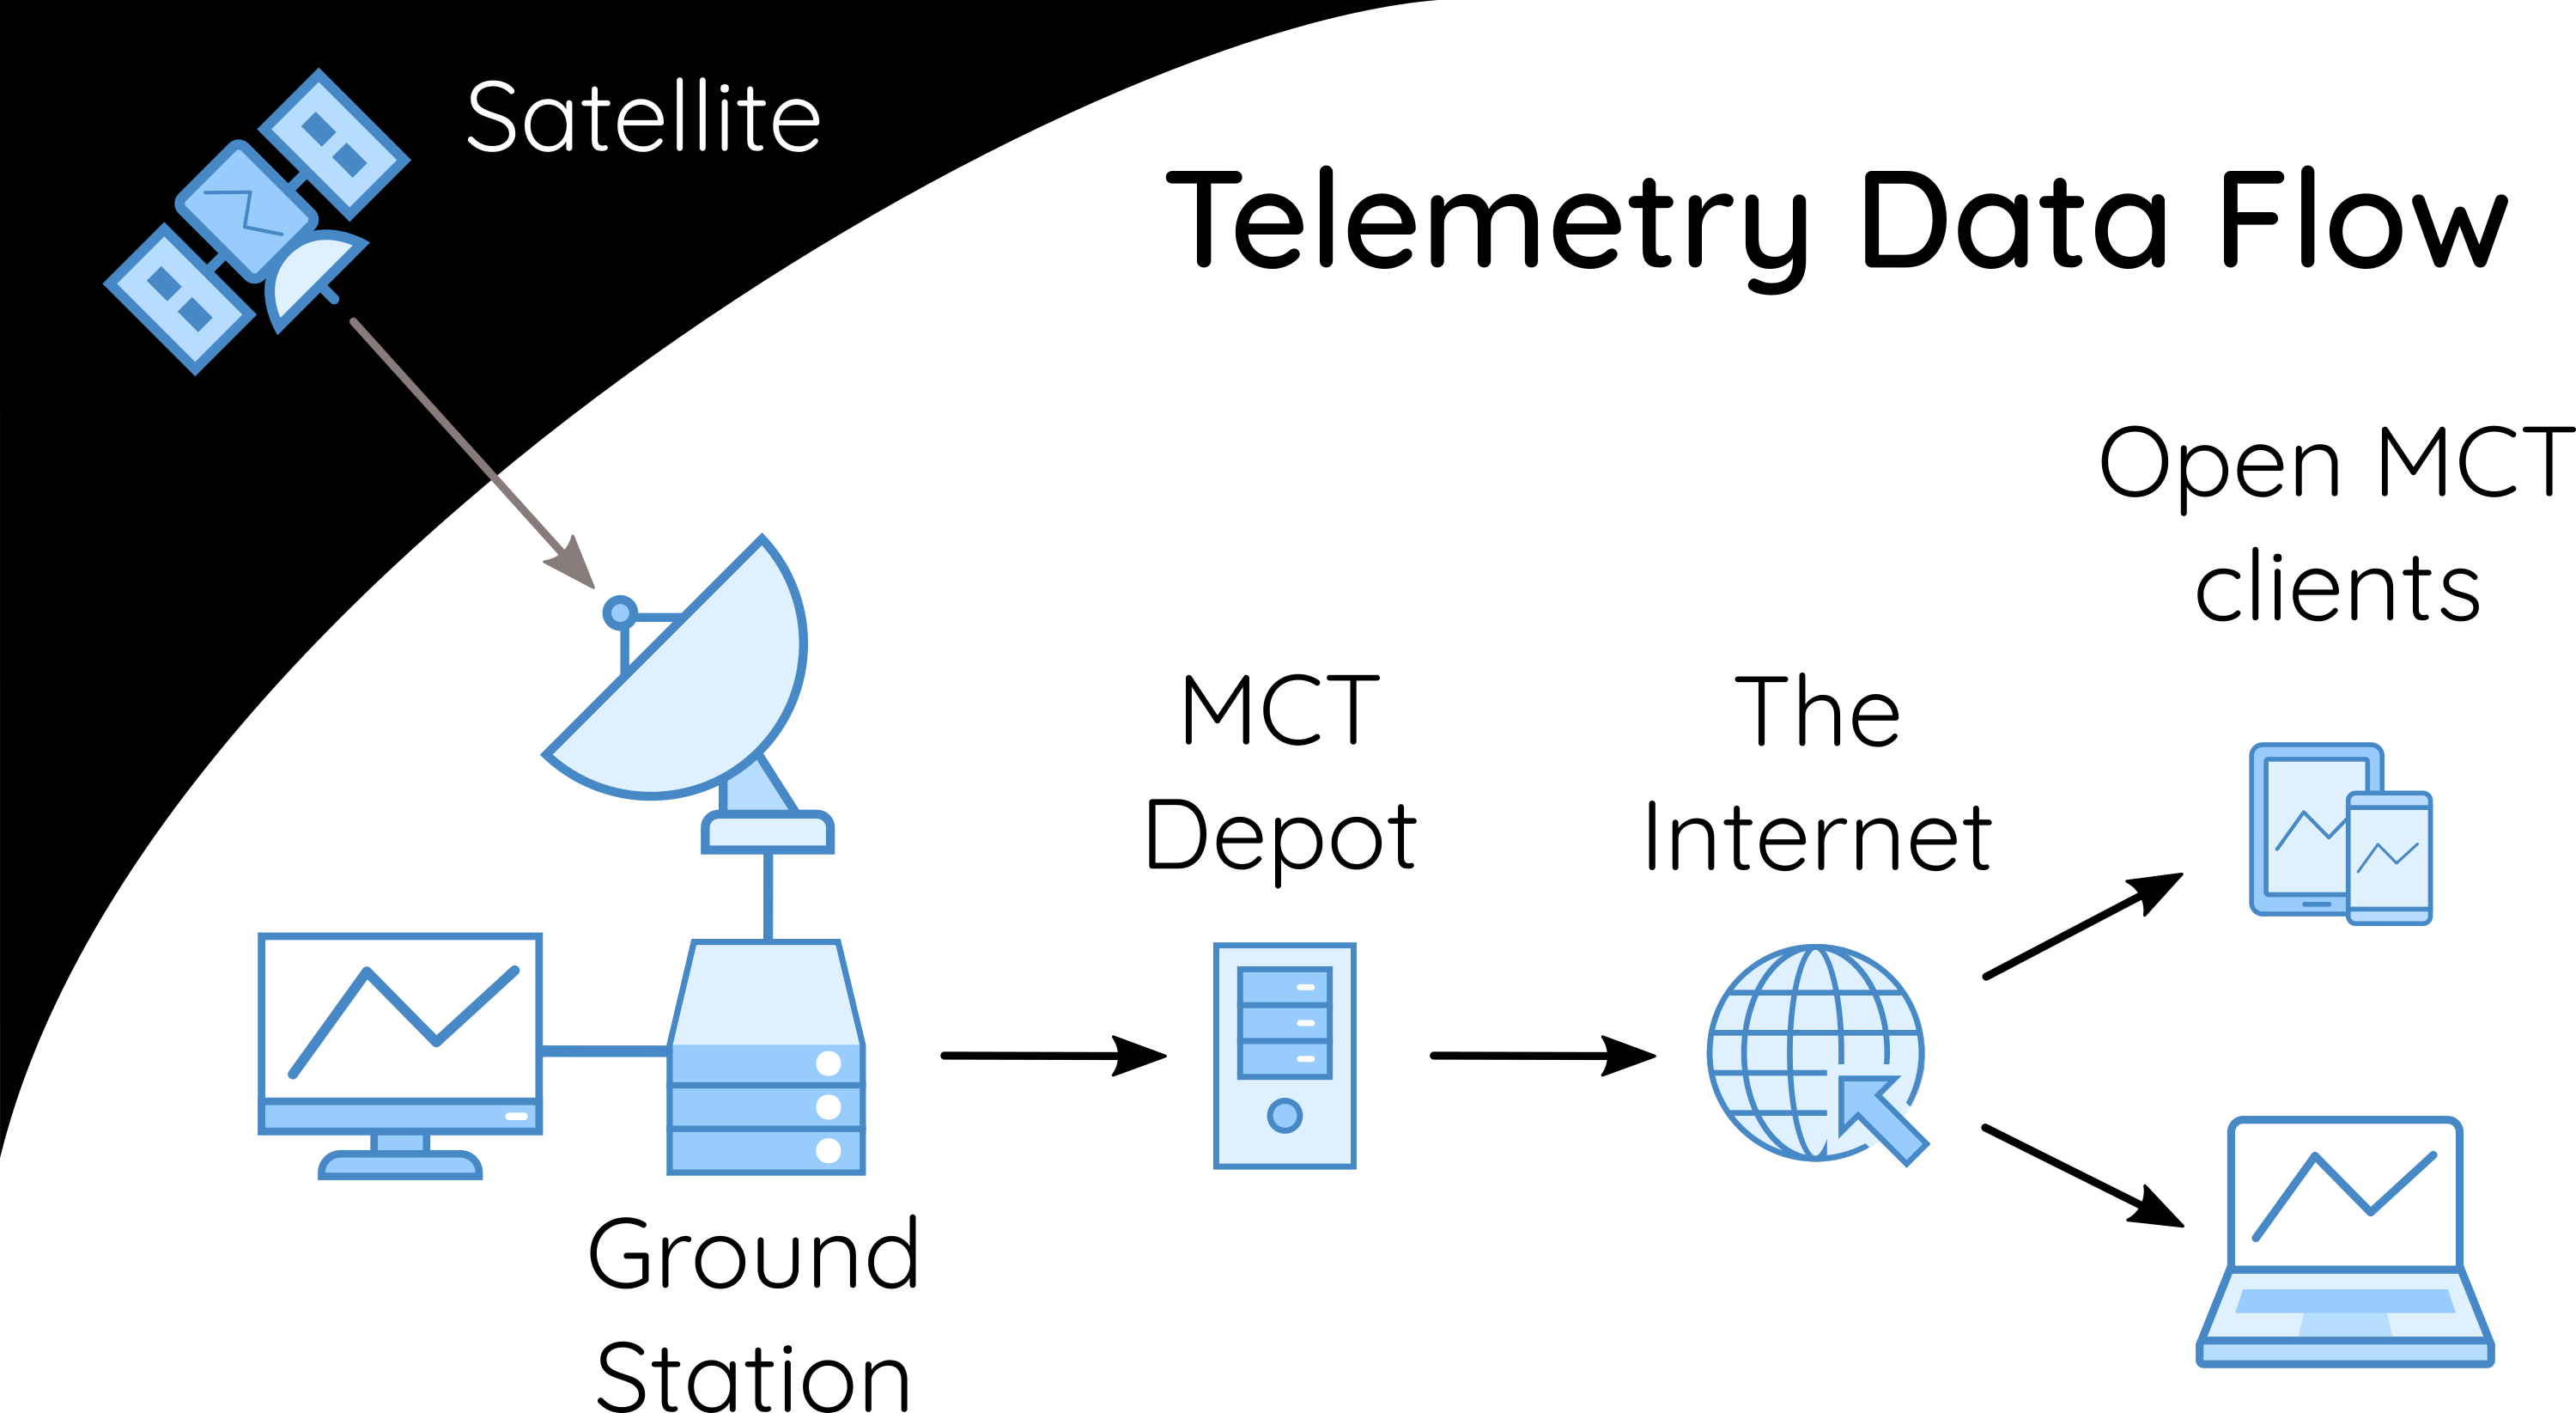
\includegraphics[width=0.7\linewidth]{Images/Diagrams/Telemetry Data Flow}
    \caption{Data flow in the proposed Open MCT-based telemetry visualisation system}
    \label{fig:telemetryflow}
\end{figure}

This is the kind of telemetry that will be the main focus of this project assignment. It usually consists of basic measurements done by the spacecraft on its hardware components, and allows ground station operators to view vital physical parameters for mission planning such as on-board power usage and generation, temperatures, position and attitude. Another common component of spacecraft telemetry is the state of its software, with important flags, variables and counters often being transmitted to let the operators know what it is doing. An example of a display showing this type of telemetry from a \Gls{cubesat} is seen in Figure \ref{fig:funcube}.

\begin{figure}[ht]
    \centering
    \includegraphics[width=1\linewidth]{Images/funcube-overview.png}
    \caption{Telemetry display from the FUNcube-1 educational CubeSat \cite{funcube}}
    \label{fig:funcube}
\end{figure}

Satellite telemetry visualisation systems commonly start at the satellite and end at a ground station, as seen in the first step in Figure \ref{fig:telemetryflow}, where one or more operators can view telemetry from the satellite and potentially send commands back. The HYPSO mission at NTNU wants to extend this to make telemetry data more readily accessible to team members and potentially external users outside the ground station using Open MCT, as seen towards the right in Figure \ref{fig:telemetryflow}.

\subsection{NTNU HYPSO}
The \acrshort{hypso} mission is primarily a science-oriented technology demonstrator. It will enable low-cost and high-performance hyperspectral imaging and autonomous on-board processing that fulfil science requirements in ocean colour remote sensing and oceanography.

\begin{figure}[ht]
    \centering
    \includegraphics[width=0.9\linewidth]{Images/ImagingSession.jpg}
    \caption{Illustration of a typical HYPSO ocean imaging session}
    \label{fig:imaging}
\end{figure}

\acrshort{hypso} will be the first SmallSat launched by NTNU, with launch planned for Q4 2020 followed by a second mission later. These are part of a vision to provide a constellation of remote-sensing SmallSats, adding a space-based asset platform to the multi-agent architecture of \acrshort{uav}s, \acrshort{usv}s, \acrshort{auv}s and buoys that have similar ocean characterisation and monitoring objectives as illustrated in Figure \ref{fig:ocean}.

\begin{figure}[ht]
    \centering
    \includegraphics[width=0.75\linewidth]{Images/Coord-1.png}
    \caption{Coordinated multi-agent ocean-sensing architecture}
    \label{fig:ocean}
\end{figure}

The \gls{satbus} and launch provider for the mission is \Gls{nanoavionics}, which also provides various other services such as telemetry storage and telecommand tools through their Mission Control Software package.

\subsection{Open Mission Control Technologies}
Open Mission Control Technologies (hereafter referred to as \say{Open MCT}) is a new mission control framework for visualisation of various types of data inside a web browser, both on mobile and desktop devices. It is actively developed as open source software at \acrshort{nasa}'s Ames Research Center, in collaboration with the Jet Propulsion Laboratory. 

\begin{figure}[H]
    \centering
    \includegraphics[width=1\linewidth]{Images/mct_demo.png}
    \caption{Sample Open MCT-based telemetry view}
    \label{fig:omctdemo}
\end{figure}

It is very flexible and extensible, allowing for many different types of data to be integrated and easily accessible on one single website for mission planning and \gls{telemetry} data analysis. It reduces the need for mission operators to switch between many different applications to view all necessary data. \cite{dev_interview, mctos}

Another large advantage of Open MCT as a telemetry visualisation system is that it allows end users to customise and share their own telemetry views without complex programming. This opens up for quick adaptation to unpredicted use cases that would commonly require significant time investment by programmers in more traditional telemetry visualisation systems; instead, Open MCT allows end users to access all its data how and when they want. This is enabled by the many plugins available by default in Open MCT \cite{mctplugins}, providing multiple ways to display data using graphs, lists and tables, in addition to providing data export functionality right out of the box. \cite{omct_intro}

Plugins are also the main way for developers to add new functionality to Open MCT, such as adding a new telemetry source to display. Where this telemetry is provided from and over which protocols is not an explicit part of the Open MCT specification, but plugins are instead expected to register providers - special JavaScript functions, with specified inputs and outputs - for certain data types. These specify how Open MCT may request and receive that data, and how it can display it.

\begin{figure}[H]
    \centering
    \includegraphics[width=1\linewidth]{Images/value_view.png}
    \caption{Sample Open MCT-based telemetry view, single value}
    \label{fig:omctvalue}
\end{figure}

A high-level overview of the providers implemented as part of a typical Open MCT plugin for a custom telemetry source is the composition provider, object provider and telemetry provider. The composition provider defines where each value is located in the object tree on the left-hand side in Figure \ref{fig:omctvalue}. The object provider essentially maps metadata for each value to a JavaScript object Open MCT can understand (see Source Code \ref{code:mct_metadata}), which allows it to use values received from a telemetry provider - either in real-time or on request - to display a graph or other visualisation.

%The framework went through a major version update during 2018-2019, resulting in numerous changes that made much of the available tutorials, documentation and earlier project reports outdated as of the writing of this report.

\subsection{Existing implementations}
There are few current users of Open MCT which make their implementations available to the public, but it is used widely within \acrshort{nasa} and \acrshort{jpl} for both space-based and terrestrial applications, with some of the more recognisable names being the Mars 2020 rover Perseverance, Mars Cube One, ICESat 2 and the Cold Atom Laboratory. LightSail 2 is an example of a high-profile non-\acrshort{nasa}/\acrshort{jpl} external user of Open MCT. \cite{omct_users}

Some of the more well-documented recent Open MCT implementations will be briefly introduced below, with most detail being given to the Open MCT project's official tutorial which is the common starting point for all of them.

\subsubsection{Open MCT tutorial}
This is the current reference Open MCT implementation, and the easiest way to get started with the framework as the current documentation can be somewhat lacking or confusing to start with from scratch.

\Gls{node} and \Gls{express} is used to implement a telemetry web server that simulates a simple spacecraft. It provides telemetry for it as \acrshort{json} over \acrshort{http} for historical data, and over \Gls{ws} for realtime data.

In Open MCT a plugin (called the \say{dictionary plugin}) is used to load the metadata specifying how the each data point in the telemetry should be displayed and acquired from the server. Two separate plugins provide the actual implementation of the \acrshort{http} and \Gls{ws} clients that interface with the aforementioned web server.

%A quick overview of the data flow in the example setup is shown in Figure \ref{ for reference.

\subsubsection{CloudTurbine}
CloudTurbine - a NASA-supported data streaming service - has made a prototype interface for Open MCT to test various aspects of how their service can be used with it.

Their prototype is a direct fork of the Open MCT tutorial repository. They have developed what they call a \say{telemetry generator layer} in Express between the CloudTurbine service and Open MCT, with the generator layer querying their backend for new data and supplying it to Open MCT as JSON over a \acrshort{http} or \Gls{ws} connection. \cite{cloudturbine}

\subsubsection{ROSMCT}
ROSMCT uses Open MCT to provide data and telemetry visualisation for Robot Operating System (ROS) robots. It consists of three distinct components, with a Rosbridge node (which provides a \acrshort{json} \acrshort{api} for ROS) running on the ROS instance to collect data from, a web server that collects data from Rosbridge, and finally an Open MCT plugin that allows the data to be displayed in Open MCT.

The web server in between Open MCT and the Rosbridge node does not have any local telemetry storage, and only provides access to realtime data from the ROS instance. \cite{rosmct}

\subsubsection{Other implementations}
A select few other interesting public uses of Open MCT that unfortunately couldn't get a full description in this report can be found in the list below.

\begin{enumerate}
  \item \url{https://bergie.iki.fi/blog/nasa-openmct-iot-dashboard/} - Uses Open MCT to display IoT device data
  \item \url{https://github.com/hudsonfoo/kerbal-openmct} - Directly requests data from a Telemachus server instance inside KSP from an Open MCT plugin, no dedicated server/middleware
  \item \url{https://github.com/SDRPLab/yamcs-openmct-plugin} - Directly requests data from a Yamcs server instance in an Open MCT plugin, no dedicated server/middleware
\end{enumerate}